\documentclass[14pt]{beamer}
\usetheme{default}
\setbeamertemplate{navigation symbols}{}
\usepackage{graphics}
\usepackage{array}

\title{Paxos on (a) many-core platform(s)}
\author{Motiejus Jak\v{s}tys \\
1003704j}

\date{March 2013}

\begin{document}

\begin{frame}[plain]
    \titlepage
\end{frame}

\begin{frame}
    \frametitle{Table of Contents}
    \tableofcontents[currentsection]
    Interrupt any time.
\end{frame}

\section{Changes in many-core platforms}

\subsection{Laws}

\begin{frame}{Laws}
    \begin{tabular}{cm{0cm}}
            Pollack's rule &
            \pause
            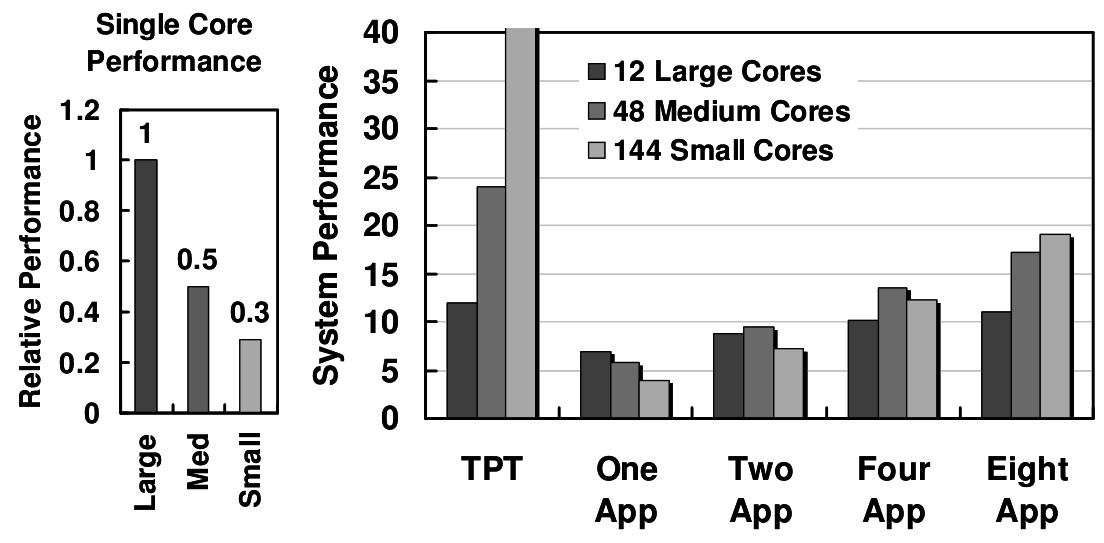
\includegraphics[height=0.4\textheight]{images/pollack.png}
            \\
            Amdahl's law &
            \pause
            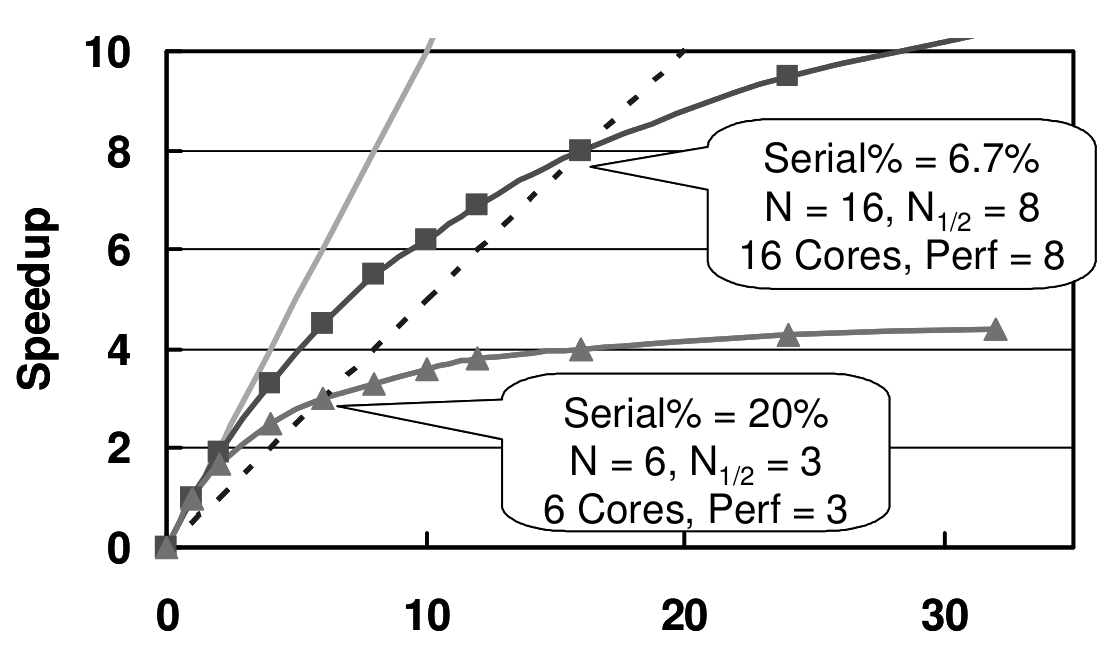
\includegraphics[height=0.4\textheight]{images/amdahl.png} \\
    \end{tabular}
\end{frame}

\begin{frame}{So?}
    \begin{itemize}
        \item Increase number of cores.
        \item And make them smaller.
            \pause
        \item \alert{Increase parallelism}
    \end{itemize}
    
\includegraphics[height=0.2\textheight]{images/orly.jpg}
\end{frame}

\section{Trends}

\begin{frame}{Tilera}
    \pause
    \begin{center}
        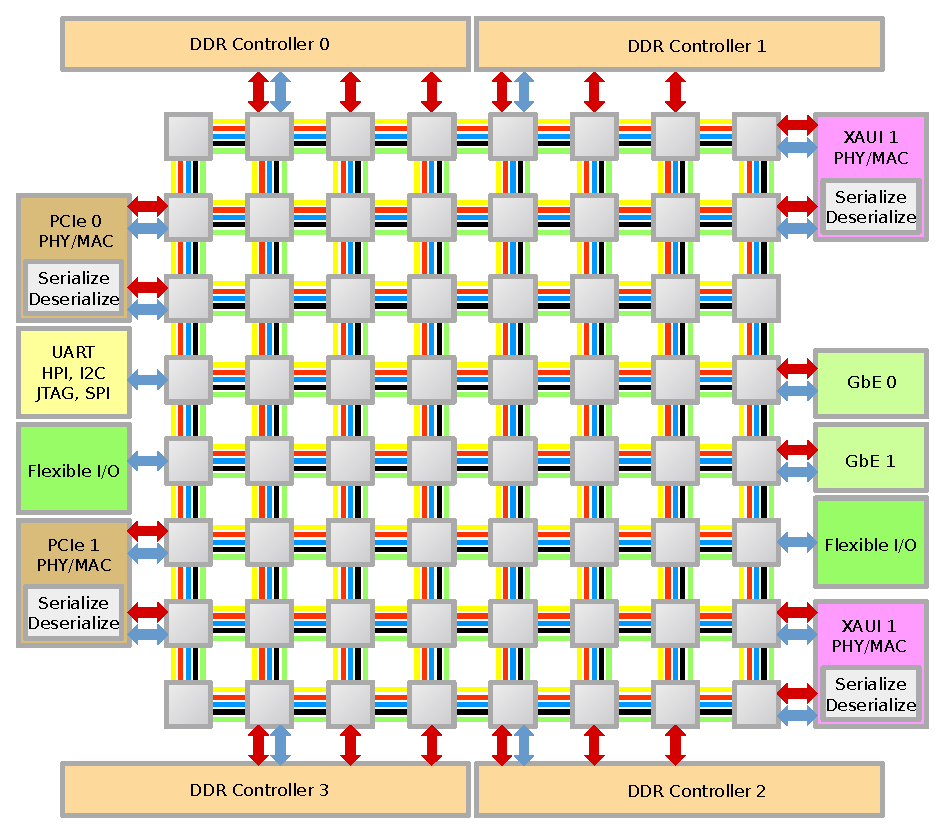
\includegraphics[height=0.8\textheight]{images/tile64.pdf}
    \end{center}
\end{frame}

\begin{frame}{Cluster?}
    \begin{center}
        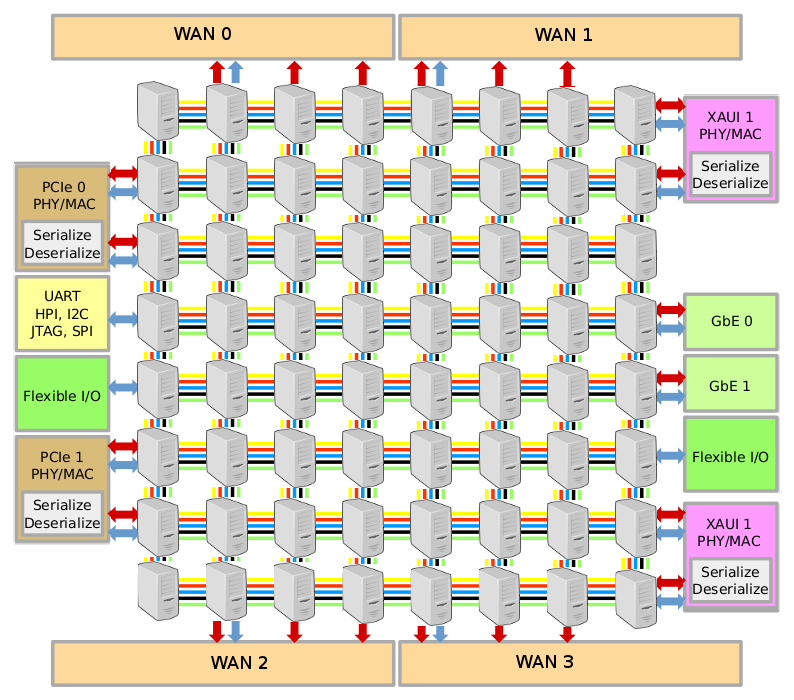
\includegraphics[height=0.8\textheight]{images/computer_clusterb.png}
    \end{center}
\end{frame}

\begin{frame}{More trendy hardware}
    \begin{center}
        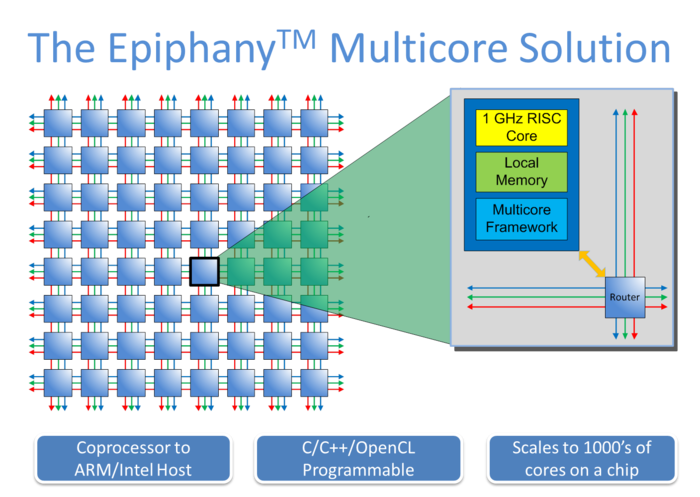
\includegraphics[height=0.8\textheight]{images/parallella_64core.png}
    \end{center}
\end{frame}

\begin{frame}{Even less chips}
    \begin{center}
        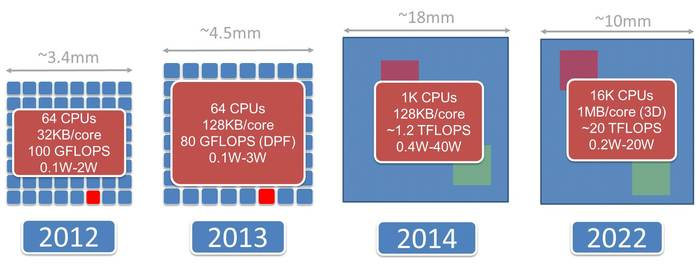
\includegraphics[width=\textheight]{images/parallella_future.jpg}
    \end{center}
\end{frame}

\begin{frame}{Recap}
    \begin{itemize}
        \item Reduce serial component
        \item Parallelization is complex to program (elaborate!)
            \pause
        \item Need redundancy to be robust
    \end{itemize}
\end{frame}

\section{Paxos}

\begin{frame}{Paxos}
    \pause
    \vspace{0.35cm}
    \hskip0.6cm
    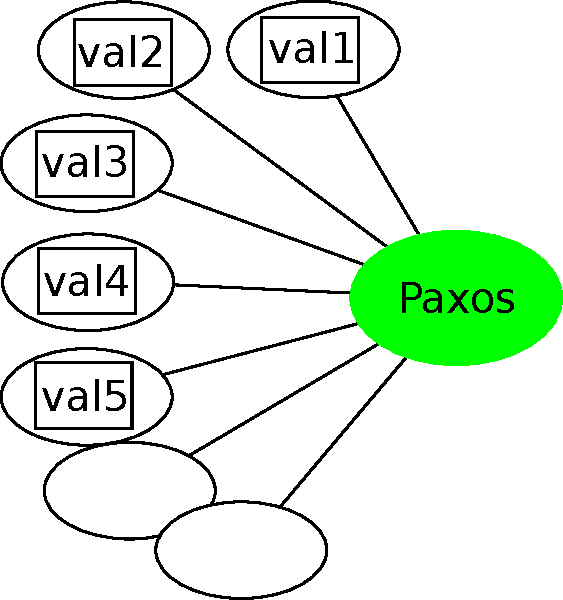
\includegraphics[height=5cm]{images/paxos1.pdf}
\end{frame}

\begin{frame}{Paxos}
    \vspace{0.35cm}
    \hskip0.6cm
    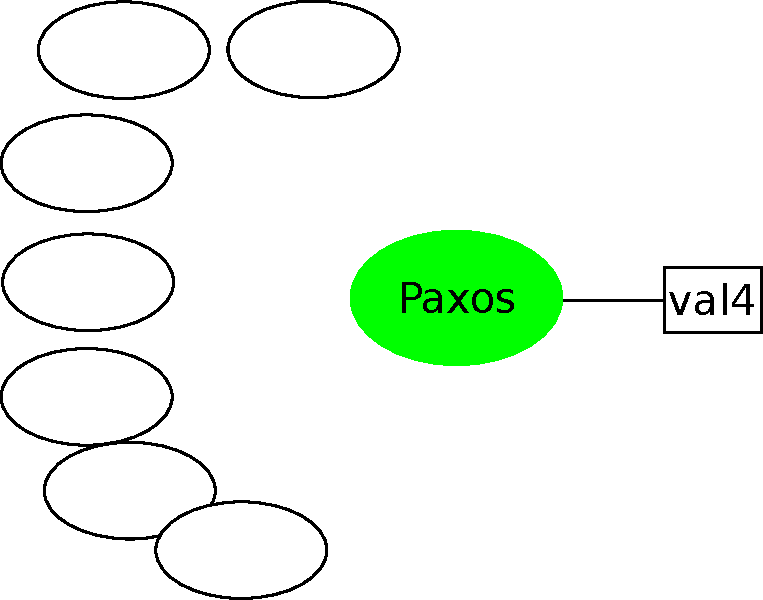
\includegraphics[height=5cm]{images/paxos2.pdf}
\end{frame}

\begin{frame}{Paxos}
    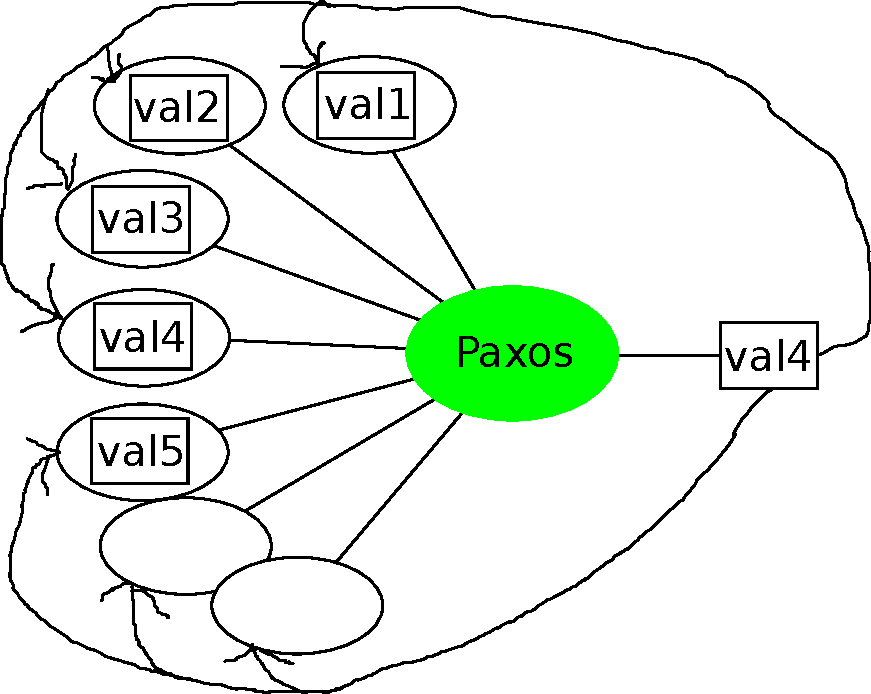
\includegraphics[height=5.87cm]{images/paxos3.pdf}
\end{frame}

\end{document}
